\chapter{行波管是怎样制造出来的?}
我们知道,行波管是依靠电子与高频场之间的能量交换来实现微波放大的一种器件。为了保证能量交换的顺利进行,我们必须给它们创造一个良好的工作环境,这个良好的工作环境就是真空。且不说发射电子的阴极根本无法在空气中工作,即使阴极能够在空气中发射出电子的话,电子在运动的过程也要不断地与大量的空气分子碰撞,结果弄得“寸步难行”,当然更谈不上得到有规律的电子流并进而与高频场交换能量了。因此,真空是行波管正常工作的首要条件,离了它什么都谈不上。


由于行波管是一种比较复杂的电真空器件,它的大部分零件都要在真空环境中工作,因此它的生产工艺流程长,需要采用一些特殊工艺和多种专用设备,而且对工艺卫生的要求很高。不同类型的行波管,它们的生产工艺往往差别很大。本章将以微波通信设备中常用的中小功率金属陶瓷行波管为例,简略地介绍其生产过程。

\section{生产一只行波管要经过多少道工序?}

图\ref{ch2-1}是微波通信设备中常用的一种中小功率行波管的结构示意图。这种行波管一般采用金属陶瓷管壳、螺旋线型慢波结构和周期永磁聚束系统。它的五个组成部分的结构和作用,已在第二章中作了简单介绍。我们还在第三章和第七章中专门介绍了螺旋线慢波结构和周期永磁聚束系统。这里想再补充一点,就是为什么要采用金属一陶瓷结构?


与玻璃结构相比,金属一陶瓷结构有下面几个优点:(1)陶瓷在高频高温下的介电损耗小。(2)能耐高温到700°C以上,因此可以提高管子的去气温度,使管内去气(关于去气,将在后面介绍)更加彻底,从而更好地保证管子的正常工作,延长管子的寿命。(3)机械强度高,使整个管子的抗冲击、耐震、可靠性能大大提高。(4)能加工成精密尺寸的零件,因此比玻璃易于保证装配尺寸,提高管子质量。(5)绝缘性能比玻璃好,可做成迭片式电子枪,如图\ref{ch10-1}中所示。在这里陶瓷环既是极间绝缘零件又是管壳密封零件,因此可以减小整个管子的体积。(6)陶瓷的导热性能比玻璃好得多,因此金属陶瓷结构更适于工作在大功率情况下。
\begin{figure}[phtb]
	\centering
	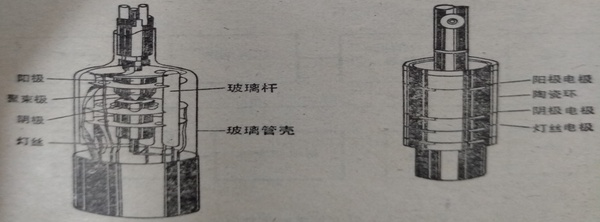
\includegraphics[width=0.8\linewidth]{figure/ch10-1}
	\caption{ 玻璃管壳电子枪和金属陶瓷电子枪的比较}
	\label{ch10-1}
\end{figure}


金属一陶瓷结构的缺点是:(1)不透明,因此不能看到管内零件的装配、对中情况,也不能用偏光仪来检验封接件的应力状况。(2)加工工序多,工艺复杂,难度大,成本高。图\ref{ch10-1}是玻璃管壳电子枪和金属陶瓷电子枪的比较。


人们还常常把行波管分成这样两个部分:(1)真空部分,即管内部分。它包括金属管壳、陶瓷窗、陶瓷环、收集极等金属、陶瓷零件构成的密封外壳以及螺旋线、夹持杆、电子枪等全部管内零件。真空部分在制造上的特点是:为了保证行波管的正常工作,管内需要保持高真空状态,所以零件都需经过严格的清洁处理,工艺卫生要求高,全部焊缝都应有可靠的真空密封性能。此外,零件加工精度、装配精度的要求也比较高。(2)非真空部分,即管外部分。它包括磁聚束系统、信号输入输出装置、散热器、电极引出线及外包装体等。这些零件虽然在清洁处理方面的要求不如管内零件高,但是,它们在加工精度、装配精度方面的要求也并不低。


行波管生产的工艺流程,从零件加工开始算起,一直到生产出一只合格的产品止,需要经过数百道工序。归纳起来可分为八个过程,如图\ref{ch10-2}所示。



\begin{figure}[phtb]
	\centering
	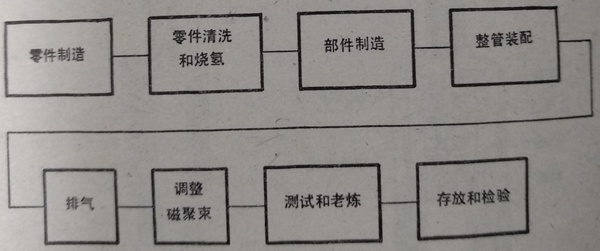
\includegraphics[width=0.75\linewidth]{figure/ch10-2}
	\caption{ 行波管生产工艺过程}
	\label{ch10-2}
\end{figure}

\section{零件制造?}
零件制造是行波管生产的开端。由于管子的零件很多,各个零件在行波管中的作用也各不相同,因此就需要用各种不同的材料来制造它们,其加工方法差别也很大。
\subsection{种类繁多的零件材料}
以某中小功率螺旋线型行波管为例,它大约由九十余种(两百多个)零件所组成。制造这些零件不但要用许多种金属材料,而且还要用一些象陶瓷、石英、塑料这样的非金属材料。现在让我们看一看各个零件所用的材料情况


阴极材料需保证阴极在一定的温度下有良好的电子发射性能和尽可能长的寿命。人们常用镍的合金(如含镁的镍,以及含锆、钨、钙等其它金属的镍合金)作为阴极基金属,发射表面喷涂上一层三元碳酸盐(即含碳酸钡、碳酸钙及碳酸锶的混合碳酸盐),在制造过程中经适当处理后便成为发射物质。为了减小高频输能装置的损耗,它的金属零件应具备良好的导电性能,因此,常用黄铜来制作输能装置的内、外导体。而且还常在它的表面镀一层金,以保证接触良好,稳定可靠。输能装置的介质零件,通常是用聚四氟乙烯制成的,它的高频损耗小,且耐高温。


实际上,作为行波管管壳一部分的陶瓷窗也是输能装置的一部分。它是高频信号出入的门户,我们正是利用了陶瓷能让电磁波透过这个特性,使高频信号能畅通无阻地由此进出行波管壳,与管外的输能装置连通。试设想如果全部管壳都是金属的,那岂不是要把高频信号进出行波管的通路全部堵住了吗?由于陶瓷窗同时又是管壳的一部分,因此,它和金属管壳之间的封接要求就十分高。通常,我们只是让陶瓷窗两端分别和一小段金属管封接起来,构成一个小零件,如图\ref{ch10-12}中的“陶瓷窗”和“封接筒”所示,它的断面图如图\ref{ch10-3}所示,然后再把这个小零件和装有螺旋线的金属管壳焊接在一起。为了达到真空密封,就要求这一小段金属管的热膨胀系数和陶瓷的热膨胀系数尽可能接近。另外还要求这段金属管是非磁性的(下面会讲到)。考虑这两方面的要求以后,人们常常选用无磁镍铜合金或无磁不锈钢来作为这段金属管的材料。至于陶瓷窗中的陶瓷材料,在微波电子管中,从介电常数、机械强度、耐温导热等多方面考虑,通常都采用九五氧化铝瓷(其成分中含95\%氧化铝)。
\begin{figure}[phtb]
	\centering
	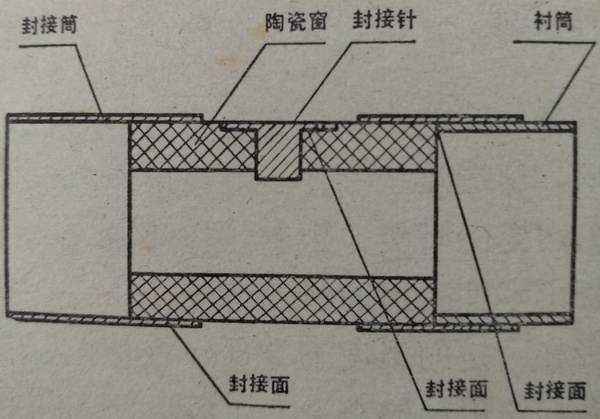
\includegraphics[width=0.6\linewidth]{figure/ch10-3}
	\caption{ 高频陶瓷窗断面图}
	\label{ch10-3}
\end{figure}

螺旋线是一种高频传输系统,但是由于它经常要受到电子为这段金属管的材能,而且应当有足够高的熔点,使它在高温下有较高的机械强度和较低的蒸发率。同时,还要求它便于加工绕制成螺旋线。钼能够较好地满足上面几个要求,因此是螺旋线的理想材料。至于螺旋线的夹持杆,我们既要求它的高频损耗小,又希望它在高温下有良好的机械强度和绝缘性能,以保证管子的正常工作,因此常常用石英或陶瓷来制作。在功率较大的行波管中,螺旋线的工作温度很高,产生的热量很多,为了使螺旋线更好地散热,还对夹持杆提出一条要求:导热性能好。因此,需要用导热性能和绝缘性能都比较好的氧化铍陶瓷来制作。


对磁聚束系统中所采用的永磁材料的要求是矫顽力高,剩磁大,温度系数小。这样就可以使整个磁聚束系统的体积和重量减小,通常采用硬磁铁氧体或高矫力的铝镍钻磁钢作行波管聚束系统的磁性材料。而对极靴和磁屏蔽零件,则要求它们的导磁率高而矫顽力和剩磁都尽可能小,通常用纯铁制作。

由于螺旋线中的电子注必须要在磁聚束系统产生的磁场作用下才能正常地与高频场相互作用,因此,整个高频系统(包括输能装置)都是处于磁场的包围之中的。为了不破坏高频系统所在处的磁场分布,就要求高频系统的所有零件全部是非磁性材料制成的。因此,金属管壳常用无磁镍铜合金制作。如前所述,陶瓷窗两端的金属管也是用无磁镍铜合金制作的。而输能装置中的内、外导体材料因为是黄铜,故已满足无磁性要求。


散热器应能把收集极的热量充分传导出来,然后散发到周围空间。因此,其零件的导热性能要好,人们常用铝和铜,更多地是用铝来制作。此外,在第八章中我们讲过,考虑到降压收集极的绝缘问题,在散热器中还应有绝缘零件,对它的要求就不仅是电的绝缘而且还需要导热性能好。人们发现,氧化铍陶瓷、氮化硼陶瓷和氧化铝陶瓷在不同程度上都能满足这个要求,在中小功率行波管中氮化硼瓷和氧化铝瓷用得更多一些。在另外一些地方,却又希望热量尽可能地不要传出去。例如,我们希望阴极的热量尽可能地少传出去,以便用较小的加热功率就能得到足够高的阴极温度(通常是~\SI{750}{\degreeCelsius}~左右)。因此,支撑阴极的零件常用导热性能很差的殷钢(一种含镍36\%的铁镍合金)来制作。


为了吸收行波管内的残余气体以提高管内真空度,管内还装置了用具有良好吸气性能的材料制作的辅助吸气部件,例如,近年来出现的锆一铝吸气剂,目前已广泛地用于生产中。

\subsection{多种多样的加工方法}
用于管内的一些薄壁金属零件,如阴极、阴极支持零件、热屏蔽零件、阳极、聚束极等,一般是以金属带为原材料,用专门的模具冲制而成的。金属带在模具中被引伸、变形,最后做成所需要的形状,如图\ref{ch10-4}所示。这种加工方法的优点是生产效率较高、用料节省,适合于大量生产。
\begin{figure}[phtb]
	\centering
	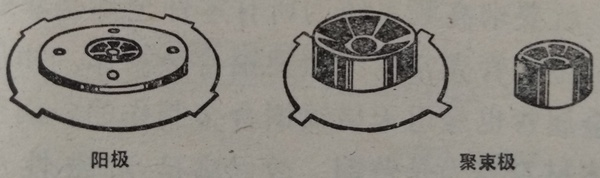
\includegraphics[width=0.65\linewidth]{figure/ch10-4}
	\caption{ 行波管的冲制零件}
	\label{ch10-4}
\end{figure}

螺旋线(或螺旋带)是中小功率行波管中的一个重要零件,其加工精度如何,直接影响到行波管的高频性能。它的加工方法是利用精密车床或专用的机床将钼丝或钼带绕在一根钼制的芯杆上,然后在氢炉中高温定形,抽去芯杆就可得到。螺旋线的内径、外径及节距都要求很严格,其公差约在百分之一毫米左右。


灯丝是个很小的零件,它的加工方法是:用很细的钨丝或钨的合金丝绕在钼质芯丝上做成单螺旋,然后把单螺旋弯成盘香或双螺旋形状,在氢炉中高温定形后再用化学方法将钼芯丝腐蚀掉。为了保证阴极和灯丝之间的绝缘(阴极与灯丝靠得很近,见图\ref{ch10-9}),最后还要在钨丝外面电泳上一层氧化铝,并在氢炉中高温烧结,才得到了图\ref{ch10-5}所示的灯丝。
\begin{figure}[phtb]
	\centering
	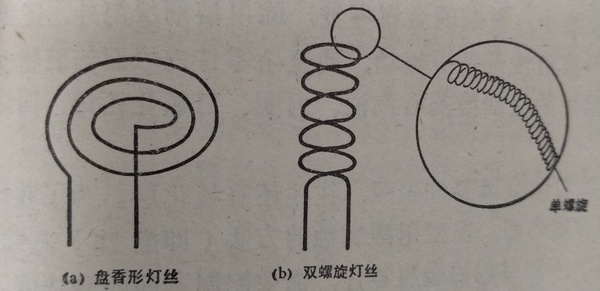
\includegraphics[width=0.7\linewidth]{figure/ch10-5}
	\caption{ 灯丝}
	\label{ch10-5}
\end{figure}

还有许多金属零件,采用的是普通的车、铣、磨等加工方法,如输能装置的内、外导体、介质支持零件等就是用车床加工的;收集极则是先经冷挤压成形后,再用车床加工的(图\ref{ch10-6});磁环的内、外圆及平面、夹持杆的外圆等,需用内圆磨床、外圆磨床、平面磨床及无心磨床来加工。
\begin{figure}[phtb]
	\centering
	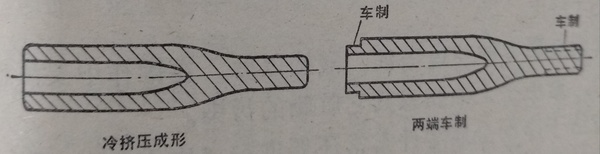
\includegraphics[width=0.7\linewidth]{figure/ch10-6}
	\caption{ 收集极的加工}
	\label{ch10-6}
\end{figure}
\section{零件的清洗与烧氢}
所有的管内零件(包括管壳),在装管以前都要进行严格的清洁处理,把它们表面的所有有机和无机脏物都去掉,这是使管子内部获得高真空度的重要一环。否则,行波管工作时这些脏物会不断释放大量气体,使管内真空度下降,以致引起阴极损坏、管内气体放电,管子无法工作。


上面说到的脏物,主要是金属零件在机械加工过程中沾上的润滑剂和金属表面的氧化层。所以,零件清洗的第一步工作是去除表面的油脂。清洗的方法很多,需要根据零件上脏物的性质及零件材料尺寸和形状来选择。例如,较大的零件可先用机械方法擦洗表面的脏物,然后再用去油溶剂浸泡,清除油层。比较细小、复杂的金属零件,除用溶剂浸泡外,还放在专门的超声波清洗设备中振动,使复杂零件内表面的脏物也能清除掉。常用的去油溶剂有汽油、丙酮、三氯化乙烯、四氯化碳等。


去油后的金属零件表面,往往还有氧化层。为了获得“新鲜”的金属表面,需要用酸腐蚀的方法(即酸洗)去除氧化层。对于不同材料的金属零件,需要配制不同的酸洗液。酸洗的持续时间一般很短,否则会使过多的金属被腐蚀掉,影响零件的尺寸精度。


管内金属零件经过去油、酸洗以后,在操作中要注意保持其清洁,避免手上油脂或其它脏物的污染。
\begin{figure}[phtb]
	\centering
	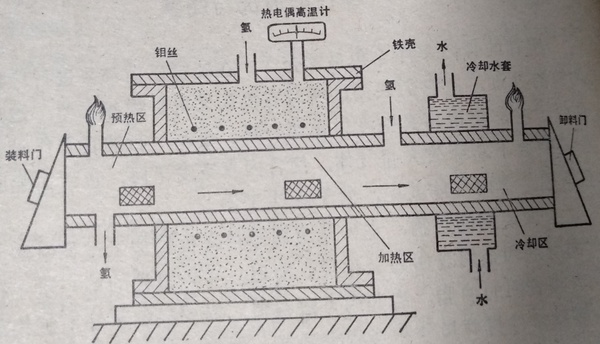
\includegraphics[width=0.75\linewidth]{figure/ch10-7}
	\caption{卧式氢炉}
	\label{ch10-7}
\end{figure}

清洁干净的金属零件常常还要进行“烧氢”处理。所谓“烧氢”就是把零件放入专门的氢炉内加热。图\ref{ch10-7}是一个卧式氢炉。氢气由管道不断流入炉管内,充满了整个炉管,然后从两端逸出炉外,因为氢气进入房间的空气中达到一定比例后会引起爆炸,所以为了安全起见,在炉管两端出口处应点燃氢气,使得跑出炉口的氢气都燃烧掉,这样,氢气就不会跑到炉外去了。同时,在炉管(通常用氧化铝瓷管制成)外面绕上电炉丝,利用电炉丝来加热炉管,使炉内温度升温到几百度到一千多度。当我们把金属零件放入氢炉中并在氢气的保护下加热(加热的温度和时间根据零件的材料和零件的大小来决定)时,由于氢气是一种还原性气体,所以金属零件不会被氧化。相反,金属零件表面的轻微氧化层会在这样的条件下被还原成金属,因此,烧氢有使零件进一步净化的作用。另一方面,烧氢还起到了对金属零件“去气”的作用。我们知道,在常温下,一切金属零件的表面和内部都分别吸附和吸收了许多气体分子,这些气体分子如果留在金属零件内部,就会在管子工作时跑出来,破坏管内真空度,使管子不能很好地工作。因此,在制造电子管的过程中,需要把金属零件内部的气体赶跑,这就叫金属零件的“去气”。在烧氢过程中,金属零件将被加热到很高的温度,此时,它所吸收的气体就会不断地从里面跑出来,因而起到“去气”的作用。不但如此,“体格瘦小”的氢气分子还能够钻入金属内部,将原有的气体分子赶跑,并取而代之,因而加速了去气的速度。烧氢完毕时,零件内部将被氢气所充满,金属零件内部气体成分的这种变化给以后的排气处理(即抽真空)带来了方便。由于一般的排气设备较易抽走氢气,因此烧氢是有利于排气过程中对金属零件的彻底去气的。

真空管壳外面零件的清洁处理要求较低,可根据不同零件的需要,先作一般清洗,然后进行电镀、油漆、氧化等处理。
\section{部件制造}
行波管在组装以前,总是把某些零件先分别组装成几个不同的部件,然后再用这些部件逐步总装成行波管。


行波管的真空部分主要包括以下几种部件:


\subsection{金属—陶瓷封接部件}


本章所介绍的中小功率行波管,它的电子枪电极系统、输入窗、输出窗都采用了金属一陶瓷封接件。图\ref{ch10-8}是金属陶瓷结构的电子枪剖面图。
\begin{figure}[phtb]
	\centering
	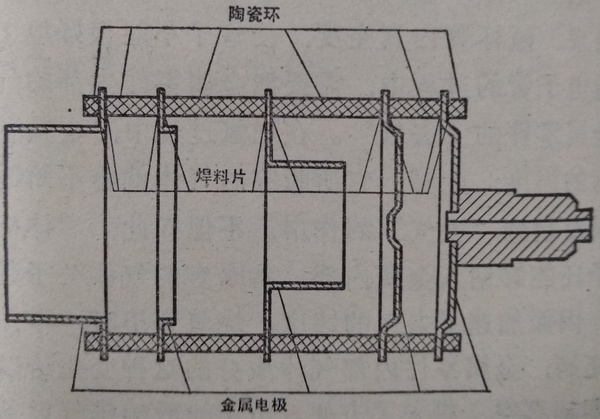
\includegraphics[width=0.75\linewidth]{figure/ch10-8}
	\caption{ 金属陶瓷封接件}
	\label{ch10-8}
\end{figure}



为了实现金属零件与陶瓷零件的密封性焊接,关键是要选择合适的陶瓷材料并在陶瓷零件的封接部分形成一层能够进行密封性焊接的金属表面(也就是陶瓷表面先形成一薄层金属层,称为陶瓷金属化)。目前微波管中应用比较广泛的陶瓷材料是九五氧化铝瓷(内含95\%的氧化铝)。常用的陶瓷金属化方法是:按一定比例将颗粒极细的钼粉、氧化锰粉、氧化铝、二氧化硅、氧化镁及氧化钙……粉末均匀地混合(这些粉末需要先经过长时间的球磨以达到一定的颗粒度)并用有机溶剂调成膏剂,涂敷在相应的陶瓷表面,然后把陶瓷零件放在氢炉中经1500\si{\degreeCelsius}左右的高温烧结,于是在它的表面就获得了一个由陶瓷到金属的过渡层。再在这个过渡层外面电镀上一层镍,这样得到的陶瓷零件就可以和金属封接了。封接的方法是把金属零件和金属化的陶瓷零件,按所要求的相对位置,放在不锈钢制成的模具内,并在待封接处放以焊料片或焊料圈(最常用的焊料是银铜焊料,其熔点是779\si{\degreeCelsius}),然后把零件和模具一同放入立式氢炉内,加温到使焊料熔化并均匀流散,即可降温冷却取出。


已经封接好的部件究竟是否能够满足真空管壳的需要,还必须经过密封性能的检验。常用的检验仪器是氦质谱检漏仪。检验方法是先将被检查的部件与该仪器连通,开动机械泵使部件抽真空,然后在部件外面的焊缝周围移动氦气喷嘴。如果某处有极小的漏气缝隙,那么从喷嘴中喷出来的氦气便由此进入部件内,并使仪器有相应的指示,这样,漏隙便被找出。密封性能不良的部件必须剔出,以免使整管报废。
\subsection{阴极、灯丝部件}

在图\ref{ch10-8}所示的电子枪电极系统中,尚未包括阴极、灯丝等零件,为了便于装配,常常将这些零件先装配成部件,然后再装入电子枪电极系统内。


阴极是电子管中发射电子的源泉,常被称为“电子管的心脏”。阴极性能的好坏对行波管的电气性能和使用寿命有极大的影响,应当作为一个重要零件而精心制作。行波管中常采用氧化物阴极,它是在清洁的阴极基金属(镍的合金制成)的表面喷涂上一层极细的碳酸钡、碳酸锶、碳酸钙的混合物而得到的。为了提高灯丝的加热效率,阴极常常制成中空的圆筒状,其顶部做成凹球面状的,是阴极的发射面,灯丝则做成盘香状的,装在圆筒内,如图\ref{ch10-9}所示。
\begin{figure}[phtb]
	\centering
	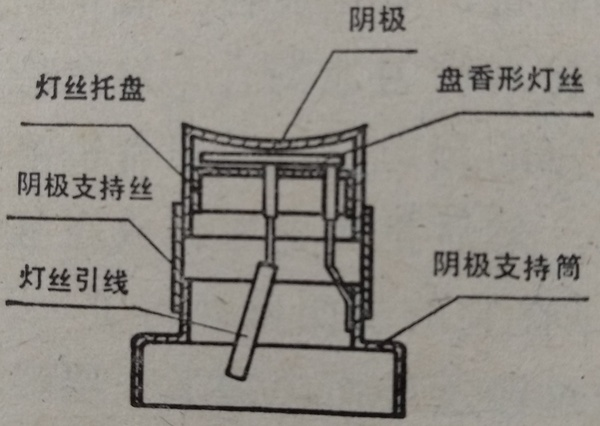
\includegraphics[width=0.45\linewidth]{figure/ch10-9}
	\caption{ 阴极、灯丝部件示意图}
	\label{ch10-9}
\end{figure}

\subsection{螺旋线部件}
为了把柔软而细长的螺旋线装入金属管壳内,并保证螺旋线与管壳良好地对中,我们常常采用介质杆来夹持、固定螺旋线。介质杆的夹持方法很多,我们已在第三章中作了介绍。这里主要谈谈弹性变形夹持法是如何实现的。图\ref{ch10-10}是弹性变形夹持法的原理图。螺旋线、介质夹持杆(常用石英杆或陶瓷杆)和金属管壳之间的相对位置如图所示。我们选择螺旋线和介质夹持杆的尺寸,使三根介质夹持杆的外公切圆的直径略大于金属管壳内径(约大0.04毫米左右)。因此,粗看起来,螺旋线和介质夹持杆是不可能直接装入金属管内的。但是,人们想出了一个巧妙的办法:先用专用的夹具把三根夹持杆和螺旋线固定在一起,夹持杆成120°地均匀分布在螺旋线周围(见图\ref{ch10-10})。另一方面,我们用三爪卡盘的三个爪夹金属管壳,使管壳稍微有点变形,因为卡盘的三个爪互相隔开120°,所以管壳受到的压力也是互相隔开120°的三点(如图中箭头所示),如果画得夸大一点的话,管壳就变成三角形的了(见图\ref{ch10-10}),这个等边三角形的外接圆直径就会比夹持杆的外公切圆的直径要大,此时就可把螺旋线和夹持杆一起推入变形的管壳中去(三根夹持杆应位于三角形三个顶部),然后撤去卡盘的压力,管壳便恢复原状,因此就把其内的螺旋线和夹持杆夹紧了。
\begin{figure}[phtb]
	\centering
	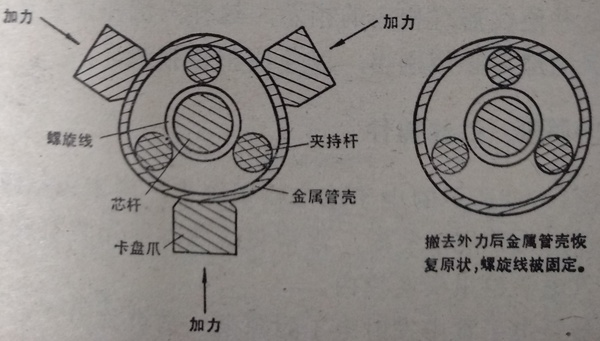
\includegraphics[width=0.73\linewidth]{figure/ch10-10}
	\caption{ 弹性变形夹持示意图}
	\label{ch10-10}
\end{figure}

夹持杆在装入管壳之前,除经过清洁处理外,还要在中间涂敷一小段碳层(或其它微波吸收材料)作为集中衰减器。我们常用“碳化”的方法来制作集中衰减器,其方法如下:在图\ref{ch10-11}所示的密封钟罩内通入正庚烷(也可用其它纯净的碳氢化合物)蒸气,在夹持杆需要碳层的位置附近用钼丝绕成的加热丝通电加热,使其周围的温度达到足以使碳氢化合物分解的温度。于是碳氢化合物在高温下就会分解出碳并附着在夹持杆表面。而在夹持杆未被加热的地方则没有碳层附着,这样就制成了集中衰减器。
\begin{figure}[phtb]
	\centering
	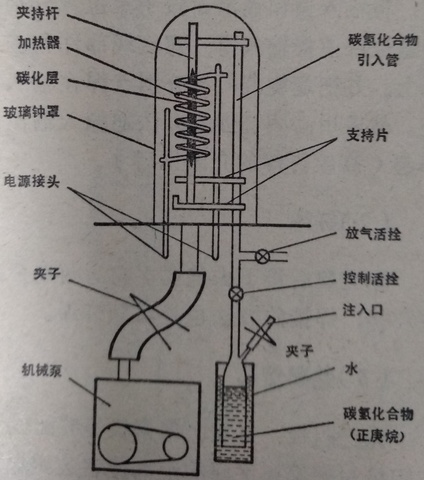
\includegraphics[width=0.52\linewidth]{figure/ch10-11}
	\caption{ 碳化装置示意图}
	\label{ch10-11}
\end{figure}
\section{行波管的装配}
上述各部件制成后,便可与其它零件一起组装成行波管了。我们结合图\ref{ch10-12}来介绍装配过程:

\subsection{配窗}

将输入窗和输出窗按予定位置分别插入螺旋线部件两端调整位置使得输入窗、螺旋线部件和输出窗三者保持在一条直线上,并把螺旋线两端分别点焊在输入窗和输出窗的金属针上。然后用高频钎焊的方法把输入输出窗和螺旋线部件焊接在一起(高频钎焊的介绍见后)。




\begin{figure}[phtb]
	\centering
	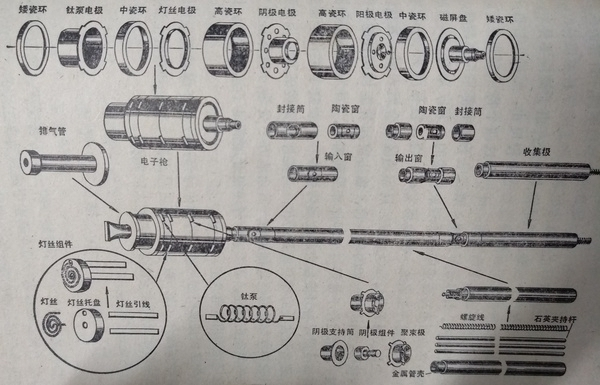
\includegraphics[angle=90]{figure/ch10-12}
	\caption{ 波导耦合型输能装置示意图}
	\label{ch10-12}
\end{figure}



\subsection{钎焊}
配完窗后接下去就要在它的两端分别与收集极和电子枪系统焊接,焊接的方法也是高频钎焊。


\subsection{装配管芯}
先把阴极、灯丝、聚束极等装配成阴极聚束极组件,并调节阴极与聚束极之间的距离使它达到规定的要求,然后和钛泵等零件一起依次装入电子枪封接件内。最后与排气管钎焊在一起,即可进行排气。为了保证管内零件不被沾污,装配过程要在卫生要求很高的房间内进行。与管内零件接触的所有工具都应清洗干净。


什么叫高频钎焊呢?和一般的熔化焊接不同,钎焊的特点是焊接时被焊金属不熔化,而是依靠熔化了的焊料来填补焊缝使被焊零件连接在一起的。钎焊的优点是:由于被焊零件不熔化,因此可以保持它原有的表面光洁度和尺寸。另外,钎焊后的焊缝具有良好的真空致密性。钎焊的这两个特点都非常适用于微波电子管。钎焊有好几种,微波电子管中都采用高频感应钎焊,它是利用高频感应的原理来焊接的。大家知道,高频电流在金属中将产生涡流,使金属发热,而且它有这样一个特点:发热仅限于受到高频感应的局部地区的金属表面,发热的速度很快。如图\ref{ch10-12}的输入窗、输出窗和螺旋线部件的钎焊过程中,我们并不希望整个零件都受到加热,因为输入窗和输出窗都是用焊料封接起来的金属陶瓷件,如果整个零件全部加热,那么封接处的焊料就要熔化,封接件就要被破坏。因此我们只希望在焊接部位局部加热,其余地方不受热,以保证整个部件的真空密封性。高频感应钎焊很好地满足了这个要求,因此被广泛地用在电真空制造中。


为了保证真空密封性,各部件每经过一次钎焊就需要用质谱检漏仪检查一次,以便及早将废品剔除,如果到整管全部装配完毕时才发现漏气就会造成更大的损失。
\section{排气}
排气是制造电子管不可缺少的一个工艺过程。我们知道任何电子管都是依靠电子在真空中的运动来工作的,因此,首先要为电子的运动创造一个真空的工作环境,这就需要把电子管内部抽成真空,这是排气的第一个任务,管内真空度的要求一般是$ 10^{-7} $毫米水银柱,也就是大气压的几十亿分之一。另一方面,为了使阴极有良好的发射电子能力,需要对阴极进行处理,也就是通常所说的阴极分解和激活,这是怎么一回事呢?原来真正能发射电子的阴极活性材料是氧化物(氧化钡、氧化锶和氧化钙),但是它们在空气中极不稳定。因此,我们就采用了这样的办法:先在空气中往金属表面喷涂一层三元碳酸盐(碳酸钡、碳酸锶和碳酸钙的混合物,它们在空气中很稳定)。然后把阴极装入管内,等到排气时抽成真空后才对阴极加热,使这些碳酸盐分别分解成相应的氧化物,例如碳酸钡分解成氧化钡和二氧化碳,后者被抽走,于是氧化钡就留在阴极表面,由于此时已在真空中,所以氧化钡就能稳定地存在。但是现在氧化钡还不具备发射电子的能力,下一步就是使它激活。激活的方法是把阴极加热到更高一些的温度,使阴极基金属中的激活剂(如镁、铝等)与氧化钡作用,还原出一部分多余的钡原子(称为盈余钡),此时阴极才具备了良好的发射电子的能力,因此,阴极分解和激活是排气的第二个任务。这个任务也是必须要在真空环境下才能完成的。排气的第三个任务是对管子的所有金属零件进行加热去气,去气的目的我们已经在前面讲过,这就是使行波管在以后的工作过程中仍然能够保持较高的管内真空度,以便使电子仍旧有一个良好的真空工作环境。为了做到这一点就必须对金属零件进行尽可能彻底地去气。在排气过程中去气是最合适不过了,因为首先,排气过程中去气的气体可以很快被抽走;其次,电子管内已抽成真空,所以就不会再有新的气体钻入金属零件中去了,只有这样才能长久地保持管内的高真空度。加热去气方法通常有以下几种:

\begin{enumerate}
	\item 烘箱加热:把整个管子置于烘箱内加热。对金属陶瓷结构的管子,通常可以加热到600\si{\degreeCelsius}左右。此时管内所有零件都受到了加热。为了防止金属外露部分在高温下的氧化,我们还把烘箱抽成低真空。
	\item 通电加热:这种加热是局部加热,例如灯丝通电就可使灯丝和阴极加热。还可以对螺旋线通电使它加热去气。
	\item 电子轰击:这种加热办法适用于某些高热零件。对于这些零件来说,光是靠烘箱的600\si{\degreeCelsius}加热去气是不够的,因为它们在行波管工作时将达到高于600°℃的温度,例如收集极就是这样。因此,对收集极我们常采用电子轰击的办法来加热去气,此时需在行波管外部套上磁聚束系统,加上各极电压并粗略地调节磁聚束系统,使得收集极电流达到一定数值,然后用控制收集极耗散功率$ P_c = I_cU_c $的办法(用改变$ U_c $的方法来控制$ P_c $)来调节收集极的加热去气功率,使收集极能够在700\si{\degreeCelsius}左右的温度下得到较彻底的去气。
	
	顺便提一点,利用电子轰击对收集极加热去气是比较麻烦的,因为它要套上磁聚束系统进行调整。过去人们常常在排气台上进行这一工作(因为收集极在去气时将放出大量气体,过去只有在排气台上才有排走这样大量气体的能力),因此就更加麻烦。近年来,利用吸气性能良好的锆一铝吸气剂已经可以使电子轰击这一工作在排气台下(也就是说在排气后)进行了,这是因为锆铝吸气剂强大的吸气能力已经使得它完全能够胜任吸收收集极放出的气体的任务了。
	
	
	利用电子轰击的办法还可以对阳极等电极进行加热去气。
	\item 高频感应加热:它的原理和高频感应钎焊是一样的。在玻璃结构的管子中,我们常常用这种办法对管内金属零件去气。
	
\end{enumerate}

排气设备通常包括三部分:(1)抽真空部分;(2)加热去气部分;(3)阴极分解激活部分,均见图\ref{ch10-13}。
\begin{figure}[phtb]
	\centering
	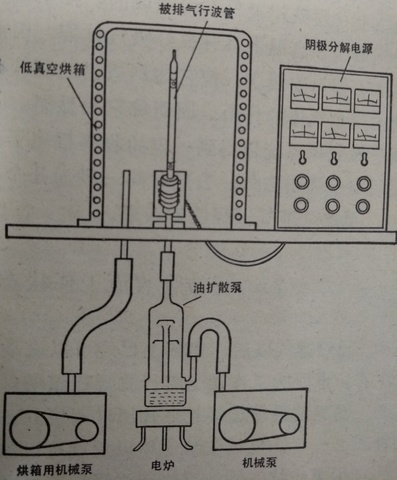
\includegraphics[width=0.6\linewidth]{figure/ch10-13}
	\caption{ 排气设备示意图}
	\label{ch10-13}
\end{figure}

\begin{enumerate}[(1)]
	\item 抽真空部分:常用机械泵和油扩散泵,后者的极限真空度一般可以达到$ 10^{-7} $到$ 10^{-8} $毫米水银柱。由于油扩散泵中的油蒸汽将对阴极产生不良的影响,因此为了使管子做到长寿命和高可靠,近年来广泛地采用了无油排气系统。
	\item 加热去气部分:主要是低真空烘箱。此外还有用来对收集极进行电子轰击去气的行波管电源。
	\item 阴极分解激活部分:主要是阴极分解激活电源。
\end{enumerate}

排气的步骤是这样的:

\begin{enumerate}
	\item 将行波管的排气管用螺母紧密地固定在排气台上。
	\item 先后开动机械泵和油扩散泵,开始抽真空。
	\item 启动烘箱机械泵,接通烘箱电源,调节其加热电流使烘箱温度升到规定数值(如600\si{\degreeCelsius}),保温几个小时。烘箱温度一般用热电偶温度计指示。
	\item 阴极分解和激活。
	\item 用冷夹钳将行波管从排气台上封离下来。
	\item 套上磁场聚束系统,启动管内辅助吸气装置如钛泵(图\ref{ch10-12}中所示的钛泵,是在碘化钛丝绕成的小弹簧外面再烧结上一层锆铝吸气剂而制成的。由于碘化钛,特别是锆一铝吸气剂,在高温下具有良好吸气性能,因此只要在钛丝中通以电流(如2安培),使它达到适当的工作温度,就能起到吸收管内残余气体的作用,因而称它为钛泵。),加上各极电压调节磁聚束系统以得到一定的收集极电子轰击功率,对收集极进行电子轰击去气,去气时间一般为几个小时。
\end{enumerate}

至此,排气过程就告结束。
\section{行波管直流工作状态的调整}
经过排气以后,实际上已经可以说基本上制成了一只行波管了。下面的工作就是将行波管和磁聚束系统、收集极散热系统、输能装置等连接起来并加以调整。它们的安装位置可以参看图\ref{ch2-1}。机械安装完毕以后就可以加上各极电压来调整它的直流工作状态了。要使行波管能够稳定地工作首先应当有稳定的直流工作状态,这主要就是电子束的调节,也就是如何把螺旋线电流调到最小,使得尽可能多的电子参予与高频场的作用,变为收集极电流。为什么行波管插入磁聚束系统后不能立刻得到良好的聚束状态呢?这是由于磁聚束系统有近百个零件,它们的加工尺寸不可能很一致,特别是磁环这样的零件,即使它的几何尺寸很一致,但是它所产生的磁场往往不可能象几何尺寸那样对称、规矩,因此由这些零件组合起来的磁聚束系统所产生的磁场就不可能是理想的轴对称磁场,它的轴线往往和行波管的轴线不一致,并且常常会产生一些有害的非轴对称径向磁场。另一方面,行波管的电子枪与螺旋线之间、电子枪中各个电极之间的对中也不可能十分理想。由于这两方面的原因,未经调整的磁聚束系统就不能产生理想的聚束效果。但是,如果调整一下磁聚束系统中的某些磁环或极靴(常用转动极靴和磁环的方法),或者在磁聚束系统外部贴上一些高导磁率的铁片,就能够改变磁聚束系统产生的磁场分布和磁场强弱,消除和减小有害的非轴对称径向磁场分量,经过这样处理以后,磁场往往能够和管子的情况对应起来,因而得到良好的电子束流通状态。这一过程通常叫做“调场”,意即调整磁场。调场的方法是先把机械安装完毕的行波管拿来,加上收集极电压和螺旋线电压,然后慢慢加大阳极电压,同时调整磁场状态,观察螺旋线电流的变化,把它调到最小。然后逐步增大阳极电压,此时收集极电流和螺旋线电流也同时增大,于是再把螺旋线电流调到最小,一直调到在规定的正常收集极电流下螺旋线电流仍然很小,这样,直流工作状态就调整完毕了。
\section{出厂前的质量检验}
为了满足整机对行波管的电气性能要求,保证使用时性能稳定、可靠,管子出厂前必须经过严格的质量检验。

\subsection{测试}
行波管的电气参数测试是质量检验的重要环节。直流参数、聚束性能应全部合格。不同类型用途的行波管,其高频参数的测试项目各有侧重。如通信用中小功率行波管的工作频段、输出功率、增益、噪声及非线性参量等都需要严格检验。各高频参数的测试方法,将在下一章中介绍。

\subsection{老炼}
参数测试合格的行波管在交付使用以前,一般需要在厂内先加电工作一定时间,称为“老炼”,也就是老化。其主要目的是:

\begin{enumerate}
	\item 进一步激活阴极,使其发射性能更趋稳定和提高。
	\item 对管子进行质量“筛选”,淘汰掉那些在老炼过程中聚束状态、发射性能变坏或出现其它疵病的管子,从而提高出厂产品的可靠性。
\end{enumerate}

老炼时间长短的选择需根据管子性能及对管子寿命、可靠性的要求来定。少则几小时,多则数十小时甚至上千小时不等。一般要求长寿命、高可靠性的行波管,老炼时间也比较长。
\subsection{存放}
行波管必须保证管内有良好的真空环境才能正常工作。但是构成行波管外壳的金属、陶瓷等材料,以及金属与金属、金属与陶瓷零件间的焊缝,都可能会因制造上的问题而使有些管子的外壳上残存很小的漏气隙缝,外面空气得以不断进入管内,因而使行波管性能恶化甚至损坏。这类管子的慢性漏气在1\textasciitilde2天内往往不能发现,为了尽量防止这样的管子出厂,经测试、老炼合格的管子在厂内应先贮存一定时间(如一个月或几个月)。

\subsection{复验}
存放了一定时间的管子在出厂前需要作最后一次检验称为复验。测试项目应包括其直流参数、聚束状态及主要高频参数。那些在存放期间性能变坏甚至失效的管子,将最后被挑出来并淘汰掉。至此,行波管才可作为成品入库。

\subsection{其它}
上面主要是对产品的电气性能检验。实际上为了保证行波管能满足一定环境的适应性要求,还应进行高温、低温、潮湿等气候试验及振动、冲击、运输等环境试验,这类试验一般是抽样进行的,即每隔一定时间从批量生产的行波管中抽取一定比例的管子进行试验。